\section*{Introduction}

As you might have noticed, the wireless smart sensor that you have been given for this project is made up of three different boards, as shown in Fig. \ref{fig:stack-overview}.

\begin{itemize}
    \item The \texttt{STM32L4A6 NUCLEO-144} MCU board is the one at the bottom. It handles mainly the MCU, the USB connection with your PC (ST-Link) and the user buttons. It is a MCU evaluation board designed and manufactured by ST Microelectronics.
    \item The \texttt{Sub-1GHz 868MHz RF NUCLEO} radio board is the one at the top, with the antenna mounted on the SMA connector. It sends your packets over the air to the gateway. It communicates with the MCU on the bottom board using mainly the SPI protocol. It is designed and manufactured by ST Microelectronics.
    \item The last board is the one in the middle. This is the \texttt{sensing and power-management} board that has been designed specifically for this project. Therefore, you will not find any documentation on the Internet. This guide is intended to provide you with all the details needed to use it properly. Please read it carefully and use it as much as possible to avoid any misuse that could damage the board(s).
\end{itemize}

\begin{bclogo}[couleur = gray!20, arrondi = 0.2, logo=\bcattention]{Be careful !}
Be careful when manipulating the boards: they are both mechanically and electrically fragile. In particular, take care of electrostatic discharge (ESD), always disconnect (and discharge large capacitors) before changing the electrical configuration of the board.
On the mechanical side, avoid disconnecting the board if possible, and be careful with the SMA connector of the radio.
\end{bclogo}


\begin{figure}[h!]
    \centering
    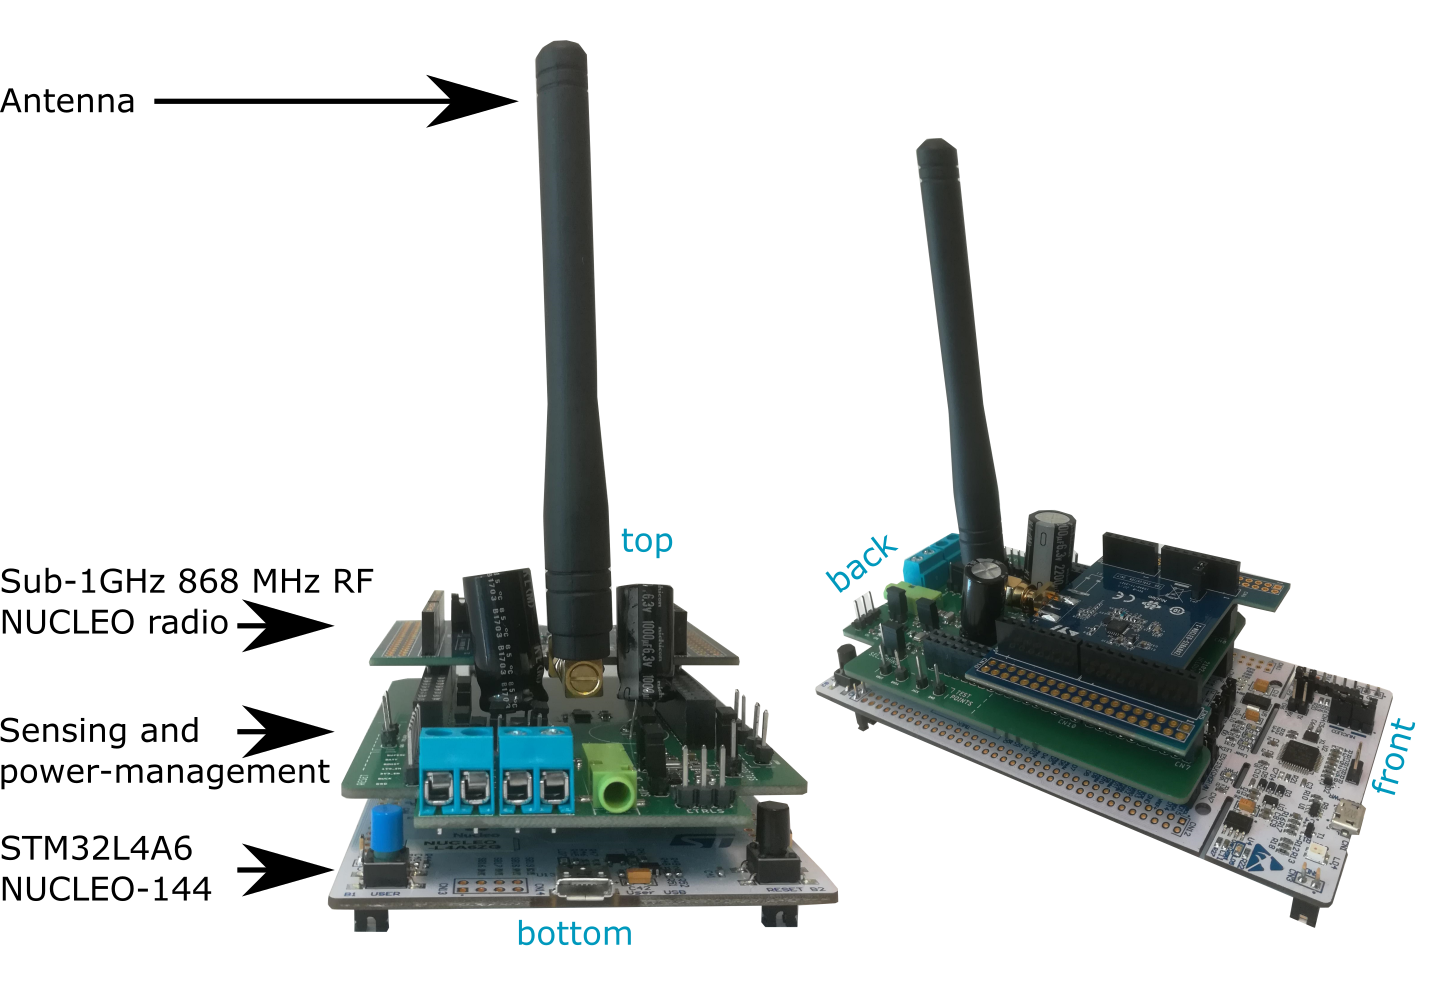
\includegraphics[width=0.7\textwidth]{figs/stack-overview.png}
    \caption{IoT node overview}
    \label{fig:stack-overview}
\end{figure}
